\documentclass[12pt, a4paper, twoside]{article} 
\usepackage{verbatim}
\usepackage{graphicx}
\usepackage{enumitem}
\usepackage{caption}
\usepackage{subcaption}
\usepackage{cleveref}
\usepackage{framed,color}
\usepackage{float}
\usepackage{listings}
%\usepackage{biblatex}
\usepackage{hhline}
\usepackage{titlesec}
\usepackage[utf8]{inputenc}
\usepackage[nottoc]{tocbibind} %Adds "References" to the table of contents
%\usepackage[numbers]{natbib}
% Tables captions set-up
\usepackage[justification=centering]{caption}
%\addbibresource{References.bib}
% Set the document margins
% Math library for equations
\usepackage{amsmath}
\usepackage[margin=3.5cm]{geometry}
\usepackage{algorithm}
\usepackage[noend]{algpseudocode}
\setlength{\parskip}{1em}

% More figures on the same page:
\setcounter{topnumber}{8}
\setcounter{bottomnumber}{8}
\setcounter{totalnumber}{8}
%bib file
\bibliography{References}
%\bibliographystyle{unsrtnat}
\definecolor{shadecolor}{rgb}{1,0,0}

\newcommand{\subf}[2]{%
  {\small\begin{tabular}[t]{@{}c@{}}
  #1\\#2
  \end{tabular}}%
}

\begin{document}


%\begin{titlepage}

\thispagestyle{empty}

\begin{minipage}{0.95\textwidth}

\newcommand{\HRule}{\rule{\linewidth}{0.5mm}}

\center 

\textsc{\large University of Southern Denmark  \\[0.4cm] Department of Engineering }\\[0.5cm] 

\includegraphics[width=3cm]{Images/SDU_logo.png}

\HRule \\[0.4cm]

{ \LARGE \bfseries [RMROVI2]Final Project:}\\[0.4cm]
\large \textsc{Object Avoidance }

\HRule \\[1.5cm]
 

\begin{center}
\small
\begin{tabular}{l}
\textit{Authors:} \\

Richárd Kemencei  \{rikem17@student.sdu.dk\} \\
Matheshwaran Pitchai \{mapit17@student.sdu.dk\} \\
Carlos Viescas Huerta \{cavie17@student.sdu.dk\} \\
Sergi Grau Moya \{segra17@student.sdu.dk\} \\

\end{tabular}
\end{center}

\vspace{5cm}


{\large \today}\\[1cm] 

%\vfill

\end{minipage}

%\end{titlepage}
% spacing: how to read {12pt plus 4pt minus 2pt}
%           12pt is what we would like the spacing to be
%           plus 4pt means that TeX can stretch it by at most 4pt
%           minus 2pt means that TeX can shrink it by at most 2pt
%       This is one example of the concept of, 'glue', in TeX
\titlespacing\section{0pt}{12pt plus 4pt minus 2pt}{12pt plus 4pt minus 2pt}
\titlespacing\subsection{0pt}{12pt plus 8pt minus 4pt}{0pt plus 2pt minus 2pt}
\titlespacing\subsubsection{0pt}{20pt plus 8pt minus 4pt}{0pt plus 2pt minus 2pt}
\newpage

\tableofcontents
\clearpage

\begin{abstract}
    This project consisted on the development of an obstacle avoidance application for a UR5 robot that is moving between two configurations. To solve it, a system integrating real time image detection and Kalman filtering alongside with dynamic online path planning was developed. 
    The robot's motion planner uses an extension of the RRT* algorithm to online planning, based on dynamic approach. It receives periodical updates of the state of the environment and detected obstacles, which is used for searching collisions along the path calculated and replan at the point of failure when needed.
    The obstacle in the scene (a red ball) is detected using a stereo camera which allows to triangulate its 3D position. Additionally, the object is tracked along the image using a Kalman Filter algorithm, which allows to keep with precision the location of the ball at any time. 
    %sum up the results
\end{abstract}
\clearpage

\section{Introduction}
\label{sec:Introduction}

In robotics, obstacle avoidance in dynamic environments is a complex problem, that requires many different sub tasks to be coordinated in order to succeed. It extends for both mobile robots and manipulators. The robot has to be able to move without colliding with other bodies, which are also moving and, in most cases, in an unpredictable way. To do that, a complex sensor system is required, capable of detecting obstacles in real time and calculating its 3D real world position. In combination with it, the planner of the robot has to be able to process this information and calculate new routes on the go.

This project, carried out during the course of Robotics and Computer Vision 2, consisted of developing an Obstacle Avoidance Application for the UR5. The robot is set to move from an initial position Q\_start to a final configuration Q\_goal, like a pick and place scenario. Then, while the robot is working, a ball is placed somewhere between the two configurations, to intentionally obstruct the initial path planning. This ball is detected using a fixed stereo camera, which is also used to triangulate its location in the 3D space, relative to the robot, and finally replan the path so that the robot avoids the ball.

Within the project, we selected two focus areas: on the robotics side, we picked On-line Path Planning. Meanwhile, on the vision side, we chose 3D object tracking using Kalman Filter.

The solution was implemented in C++ with the help of some well-known software packages. We used the robotics framework ROS to integrate all the different sub-parts. Then, for vision we used OpenCV libraries and, in robotics, we used ROS C++ API as well as the RobWork and CAROS libraries, provided by SDU. 
\newpage
\subsection{Reading guide}

The following lines describe the structure of this report. The first part of it corresponds to the explanation of the theory concepts behind the system implemented, while the second part is more focused on describing the technical details of it and the experiments carried with their results at the Lab. 

Section \ref{sec:arch} presents a general overview of the system and its architecture. Section \ref{sec:calib} explains how the camera and the robot were calibrated. In Section \ref{sec:plan}, the fundamentals of the method used for achieving online-path planning in the dynamic environment are explained. For the vision part, object detection and triangulation are described in section \ref{sec:det} and \ref{sec:tri}, while how to track it with the Kalman filter is explained in section \ref{sec:kal}. This is the end of the theoretical part of the report. Regarding the next sections, the number \ref{sec:ros} explains in deep the ROS network created to implement all the previous algorithms. Sections 8 and 9 contain the experiments carried to evaluate the system and what we obtained and, finally, sections 10 and 11 present the discussion and conclusions over the whole project.



\newpage
\section{Architecture of the system}
\label{sec:arch}
The block diagram of the system can be seen in Figure \ref{fig:arch}. The system starts calculating a initial path plan for the robot based on the initial state of the workspace. Then, periodically, the stereo camera provides two images, in which features of the ball are detected and used to triangulate the location of the ball in the real world. This triangulation is done by the epipolar lines method. This 3D coordinates are forwarded to the Kalman filter, which keeps track of the object more accurately. Once the 3D coordintate prediction is obtained, it is used for updating the environment of the robot and the collision map, in seek of potential collisions all along the path that was initially calculated.

All this information is sent to the planner of the robot, which based on it, determines if the robot can still stick to the initial plan to reach the goal or, it is necessary to replan the root to avoid obstacles that are now on the way.
\begin{figure}[H]
    \centering
    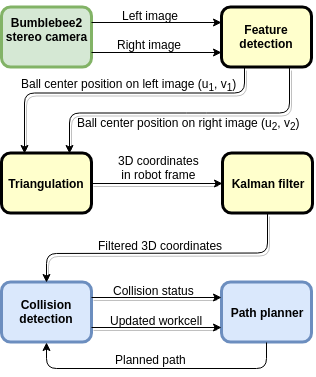
\includegraphics[width=0.7\textwidth]{Images/arch.png}
    \caption{Data flow}
    \label{fig:arch}
\end{figure}

This main structure has to be accommodated to the software used. To see the whole design of the system using ROS, go to section \ref{sec:ros}.
\section{Calibration}
\label{sec:calib}

For accomplishing the object avoidance, it is essential to determine the position of the object with a reasonable accuracy. Since our stereo camera has a fixed position in the workcell and we need the position of the ball with respect to the robot, we needed to perform an eye-to-hand camera calibration process. Our main goal was to get a fairly accurate transformation from the camera to the base of the robot. After getting this transformation matrix, the result of the triangulation can be used (which is a translation vector from the camera frame) to obtain the position of the ball in the robot base frame.\\

There are multiple ways to perform this camera calibration. We chose to go a simple way, because eye-to-hand calibration was not our focus area. Also, it's not a huge problem if we have a relatively small error in the position of the ball because we are only doing avoidance and not something which requires more precise information, for example object grasping. Furthermore, we are adding some clearance to the constructed collision area to deal with the errors originating from the quick and easy calibration process.\\

Our method was to measure the distances along the coordinate axis of the robot base with a tape measure. This gave us a rough idea about the position of the camera with respect to the robot. The orientation required a bit more work. The idea was to add a simulated camera to the provided RobWork workcell and compare the image of it with the image of the left camera of the Bumblebee.\\

\begin{figure}[ht!]
    \centering
    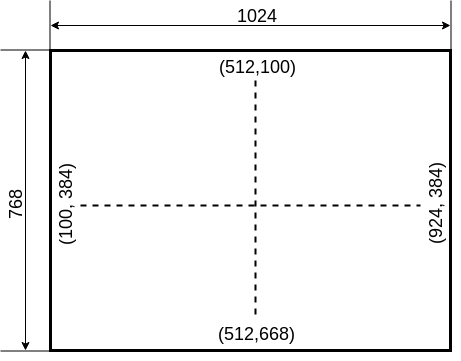
\includegraphics[width=0.6\textwidth]{Images/definedpoints.png}
    \caption{Defined cross on the image of the camera}
    \label{fig:definedpoints}
\end{figure}

We defined four points to define a cross on the picture of the left camera like on Figure \ref{fig:definedpoints}. \\

We moved the robot into such configurations where we had the TCP aligned with the defined points and recorded the 3D positions of the TCP. Afterwards, we placed four small objects into the recorded 3D positions in RobWorkStudio. We drew a cross to the picture of the simulated camera to help the alignment. The camera orientation was adjusted until we aligned the objects with the cross as good as possible.\\

\begin{figure}[ht!]
    \centering
    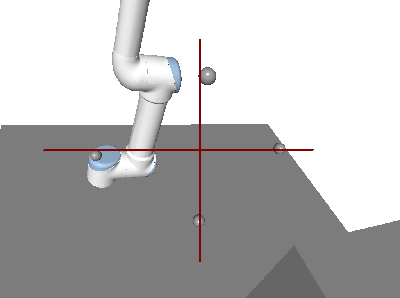
\includegraphics[width=0.6\textwidth]{Images/robwork_calib.png}
    \caption{Finding the right orientation of the camera with the help of a simulated camera in RobWorkStudio}
    \label{fig:robwork_calib}
\end{figure}

As a result, we obtained the Euler angles of the camera frame with respect to the robot base frame. We constructed a transformation matrix of these angles and the translation and inverted it using RobWork to get the final input for the triangulation program.
 \section{Motion Planning}
\label{sec:plan}
% Path planning, RRT*, anytime dynamic...
Motion planning in a dynamic environment requires agility and computational speed, such that the robot is able to check the status of the environment in cycles that allow sufficient anticipation to obstacle that are moving. A previous offline plan can be made before the operation starts, but then, the robot needs to update it with information from sensors, being able to change or replan when other bodies obstruct the trajectory.

\subsection{RRT*}
\label{sec:rrt}
The RRT* algorithm, also called RRT-connect, is an improved extension of the original RRT (Rapidly-exploring Random Tree). This algorithm is used to search for collision-free paths in high dimensional spaces, such as the Configuration Space (C-space) of the robot. Initially, it is given the \textit{map} of the C-space itself, an initial configuration \textit{Q\_start} and a final goal configuration \textit{Q\_goal}. It works by constructing a space-filling tree of nodes based on random exploration of the space, extending nodes by a fixed distance (epsilon parameter). Each node represents an intermediate \textit{Q} vector to move from start to goal. \\

The original RRT was designed to start the tree and grow only in one direction, from the starting node to the goal. RRT*, however, uses both input configurations (\textit{Q\_start} and \textit{Q\_goal)}, starting a tree in both and growing with the attempt to match both trees, which solves the path in shorter time. Figures \ref{fig:rrt} and \ref{fig:rrs} illustrate both RRT and RRT* algorithms.\\

\begin{figure}[ht!]
\centering
\begin{minipage}{.5\textwidth}
  \centering
  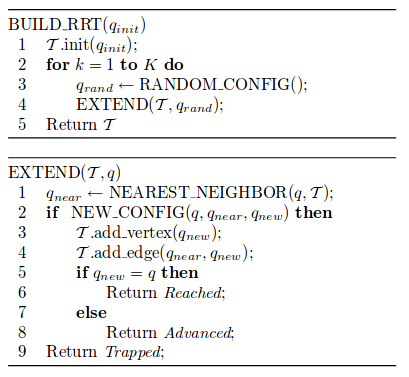
\includegraphics[width=1\linewidth]{Images/plan/RRT.png}
  \captionof{figure}{RRT algorithm. Source: \cite{RRTConnect}.}
  \label{fig:rrt}
\end{minipage}%
\begin{minipage}{.5\textwidth}
  \centering
  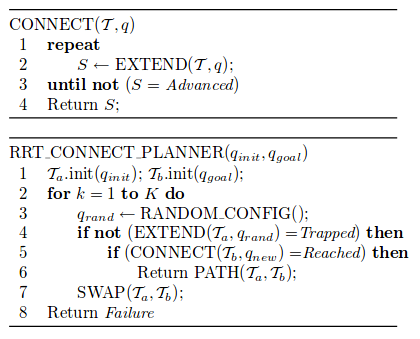
\includegraphics[width=1\linewidth]{Images/plan/RRTstar.png}
  \captionof{figure}{RRT* algorithm. Source: \cite{RRTConnect}.}
  \label{fig:rrs}
\end{minipage}
\end{figure}

The size and the run-time of the RRT* depends a lot in the size of the epsilon (extend) parameter. In operations in which the robot motion can be solved offline, and therefore there is plenty of time for the algorithm to work, RRT* tends to find optimal path solutions. However, our task is time-demanding, and therefore the path calculation time has to be kept to a minimum. The tree methodology of RRT* is very suitable for obstacle avoidance since it is able to produce solutions at anytime, but these solutions are not optimal and therefore, path optimization methods have to be used to improve the efficiency of the system.


\subsection{Online Planning}
\label{sec:onl}

The RRT* itself is not self-reconfigurating. It has no implementation of a functionality to periodically receive new environment information and update the C-space in search of possible collisions, nor the ability of replanning. To solve this problem Dynamic RRT* is used. With this improvement, it is possible to replan efficiently (without doing it from scratch) based on obstacle detection by the system's sensor. The online planner is constructed as follows:\\

\begin{algorithm}
\caption{Online Planner Dynamic RRT*}\label{planner}
\begin{algorithmic}[1]
\Procedure{Procedure}{}
\State \emph{loop}:
    \State $\textit{Initialize(Tree, q\_start, q\_goal)}$
    \State $\text{path} \gets \textit{planRRT*(Tree)}$
    \State $\textit{postSolution(path)}$
    \State $\text{obstacles} \gets \textit{findObstacles()}$
    \ForAll{$\textit{obstacles}$}
        \State  $\textit{InvalidateNodes(Tree, obstacles)}$
    \EndFor
        \If {$\textit{path} \text{ contains invalidated nodes}$}
            \State $\text{path} \gets \textit{replanRRT(Tree)}$
            \State $\textit{postSolution(path)}$
        \EndIf 
    \State $\textit{updateParameters(Tree)}$
\EndProcedure
\end{algorithmic}
\end{algorithm}

The planner starts the tree and calculates an initial path with the starting state of the workspace. As the robot starts moving, it keeps receiving data from the camera about the location of the moving obstacles. This data is processed online, and the system checks for collisions inside the path. This is done by filtering the nodes of the path in a collision detector that contrasts the position of the arm in each node with the current location of the ball (derived from the latest coordinates received from the camera). If any of this nodes is in collision, planner invalidates it, and cuts the tree at that point. Then, it replans from there a new path to the goal that avoids the obstacle. In the mean time, the collision detector keeps running and this process is repeated again if a new collision is found due to new updated locations of the obstacle.  \\

When the system does not detect collisions, and there exist already a calculated collision free path, the robot just keeps moving to the goal until the collision detector tells the contrary. This combination of RRT* and dynamic planning allows for fast replanning when necessary, otherwise fast collision free path planning for the robot to get to the goal \cite{connell}. \\

\subsection{Path Optimization}
\label{sec:opt}

As we stated previously, at fast computation times, the solutions provided by the planner are far from being optimal. Usually, these solutions contain a lot of unnecessary and/or redundant nodes along the path. In order to improve this inefficient paths, we used the optimization method called path pruning. This operation eliminates all nodes $n_{i}$ whose prior $n_{i-1}$ and posterior nodes $n_{i+1}$ are both collision free. It is a deterministic technique, meaning that it always return the same solution for the same given input state. The algorithm is shown in figure \ref{fig:prun}. \\

\begin{figure}[ht!]
    \centering
    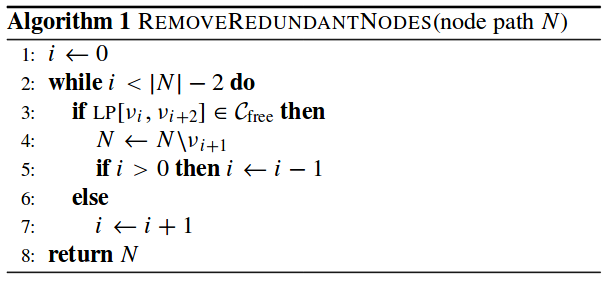
\includegraphics[width=0.7\textwidth]{Images/plan/pruning.png}
    \caption{Path pruning algorithm. Source: \cite{optimization}}
    \label{fig:prun}
\end{figure}

We chose this optimization solution over others available for several reasons. Firstly, since RRT* produces paths that are composed by a discrete sequence of nodes, pruning is a perfectly suitable complement to it. Secondly, obstacle avoidance requires computational speed, and pruning is a fast method. The main drawback of this method is that it may reduce the clearance between the obstacle and the robot. However, for that reason, the obstacle model has been already built with sufficient clearance in the radius size, to prevent from this situation. \\
 \section{Object Detection}
\label{sec:det}
The object detection part of the project consists of feature extraction and triangulation. For the robot to effectively avoid the obstacle and to plan the path accordingly, it has to know the position and orientation of the obstacle. In order to make it simple for implementation, the obstacle selected here for detection is a sphere, which makes the orientation of the obstacle unnecessary. So, the position of the sphere (x,y,z) with respect to the base frame of the robot is enough to avoid it. The feature of the obstacle is further constrained by colour, which is chosen to be red. Since the depth information is critical for the object avoidance, stereo cameras are used. Prior to using the stereo camera, it has to be calibrated accordingly. The stereo camera gives us two images of the same scene, which is essential to get the depth information. More information about the calibration process can be found in the section \ref{sec:calib} of the report.\\

The feature extraction part deals with identifying the obstacle in the 2D image frames from the stereo camera. The result of the feature extraction process is the pixel location (u,v) of the obstacle's centre (the sphere's centre) for both the left and right images of the same scene. The process is continuous and results in the same for each frame from the stereo camera.\\

The triangulation part deals with finding the position of the obstacle (x,y,z) with respect to the camera frame, making use of the intrinsic and extrinsic parameters of the stereo camera. A transformation from the camera frame to the robot's base frame will give us the position of the obstacle in the base frame.

\subsection{Feature Extraction}
\label{sec:feat}

The feature extraction process is based in color segmentation. To get results good enough, this is done in HSV space. The reason to do so is that, in HSV space, color information is separated from brightness information. In that way, we can easily threshold the image according to red color Hue values, abstracting from illumination issues, allowing only the red pixels. The resultant binary image may contain some noisy white pixels, which are eliminated by performing an opening morphological operation with an elliptical kernel. As a result of this operation, we get a binary image with white pixels only for the red ball.\\

The approach is kept as simple as possible, in order to have very low run-times. The workspace of the robot is constant, and the ball is made of a color in high contrast with everything inside it. Color segmentation is enough to provide an accurate detection. With the binary image already working, the next step is to decide which features will be used to feed the system with a point pixel of coordinates locating the ball. The main idea is to approximate its center. To do that, we find the contour of the ball's blob in the image and calculate the minimum circle that encloses that contour. This circle's center is the coordinate that the detector sends to the next phase in the vision system.\\

In figure \ref{fig:feature_extraction}, the sequence of the detection process is shown, from the starting input image to the final detection of the ball.

\begin{figure}[ht!]
\begin{subfigure}{.5\textwidth}
  \centering
  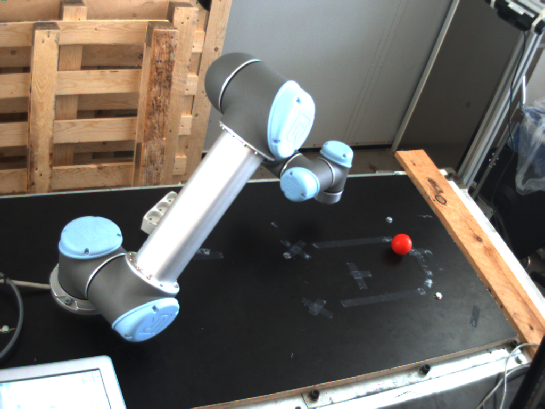
\includegraphics[width=.8\linewidth]{Images/left.png}
  \caption{Original Image Left}
  \label{fig:sfig1}
\end{subfigure}
\begin{subfigure}{.5\textwidth}
  \centering
  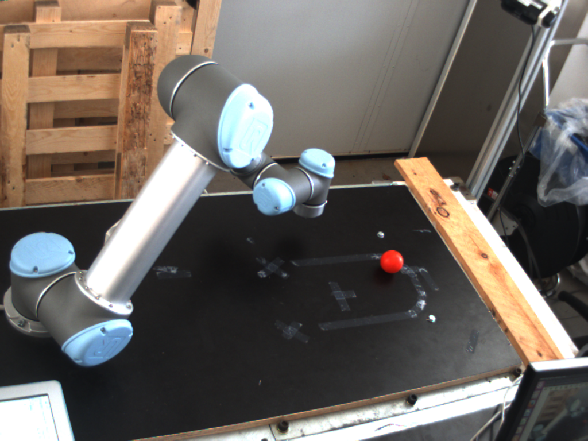
\includegraphics[width=.8\linewidth]{Images/right.png}
  \caption{Original Image Right}
  \label{fig:sfig2}
\end{subfigure}
\begin{subfigure}{.5\textwidth}
  \centering
  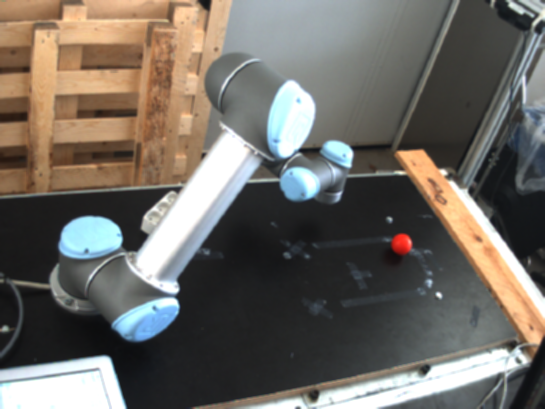
\includegraphics[width=.8\linewidth]{Images/blurred_left.png}
  \caption{Blurred Image Left}
  \label{fig:sfig3}
\end{subfigure}
\begin{subfigure}{.5\textwidth}
  \centering
  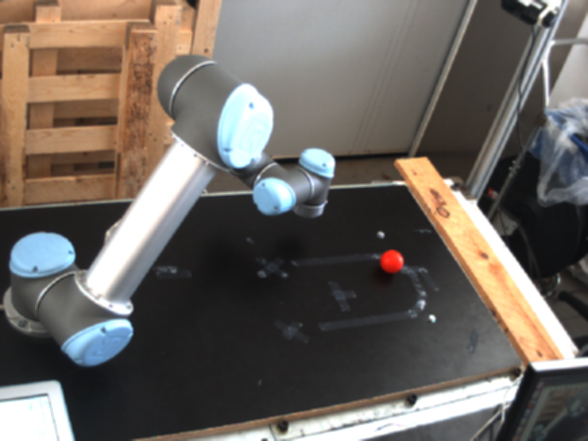
\includegraphics[width=.8\linewidth]{Images/blurred_right.png}
  \caption{Blurred Image Right}
  \label{fig:sfig4}
\end{subfigure}
\begin{subfigure}{.5\textwidth}
  \centering
  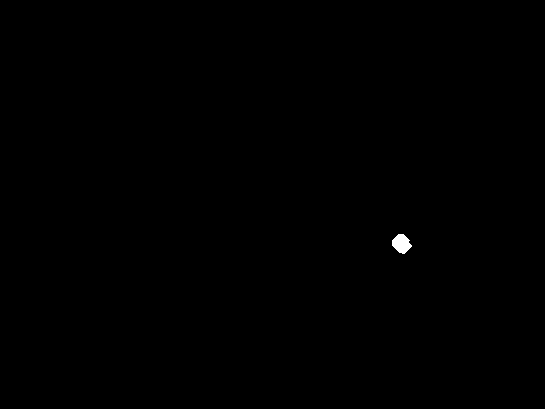
\includegraphics[width=.8\linewidth]{Images/morphed_left.png}
  \caption{Morphed Image Left}
  \label{fig:sfig5}
\end{subfigure}
\begin{subfigure}{.5\textwidth}
  \centering
  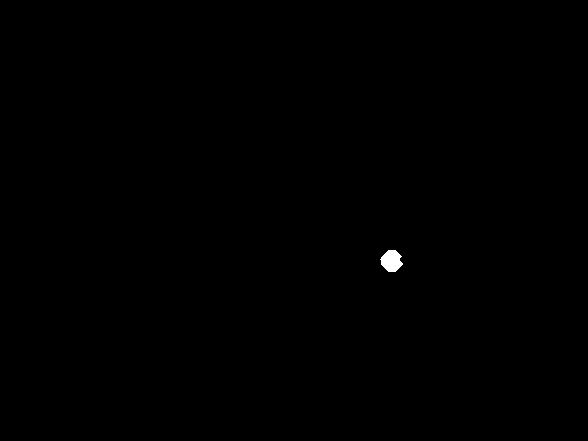
\includegraphics[width=.8\linewidth]{Images/morphed_right.png}
  \caption{Morphed Image Right}
  \label{fig:sfig6}
\end{subfigure}
\begin{subfigure}{.5\textwidth}
  \centering
  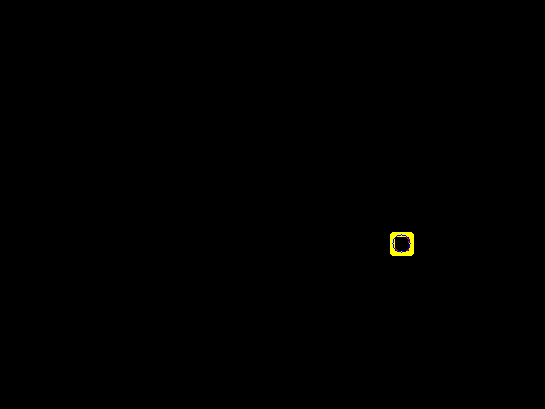
\includegraphics[width=.8\linewidth]{Images/bigbbox_left.png}
  \caption{Bounding Box Left}
  \label{fig:sfig7}
\end{subfigure}
\begin{subfigure}{.5\textwidth}
  \centering
  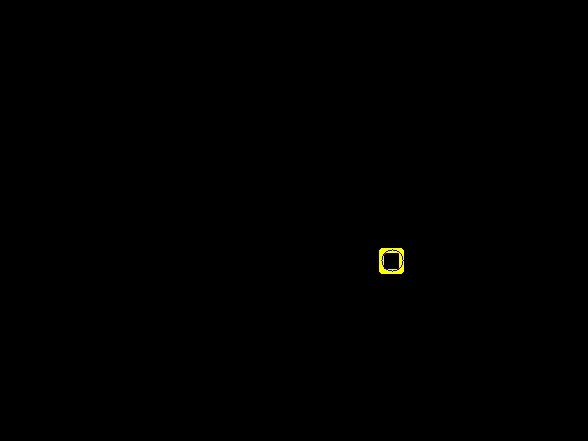
\includegraphics[width=.8\linewidth]{Images/bigbbox_right.png}
  \caption{Bounding Box Right}
  \label{fig:sfig8}
\end{subfigure}
\caption{Resultant images of the feature extraction process}
\label{fig:feature_extraction}
\end{figure}

 \subsection{Triangulation}
\label{sec:tri}

So far, we can find the location of the obstacle in the 2D images, now that we need to know the location of the obstacle in a three-dimensional Cartesian coordinate system, which is possible using stereopsis and point reconstruction. To be able to triangulate the center of the ball in 3D, we need to build the projection matrix based in the intrinsic and extrinsic parameters of both the left and right camera. This parameters were obtained in the calibration process. \\

The intrinsic matrix of the camera is a 3x3 matrix, consisting the focal lengths (fx, fy) and the principal points (Cx, Cy), which helps in projecting the 3D points in the camera coordinate frame to 2D pixel coordinates. This intrinsic camera matrix is for the raw distorted images. The distortion model of the camera and its parameters are identified in the calibration process, which can be used to get an undistorted image. The projection matrix is a 3x4 matrix with its left 3x3 portion corresponding to the intrinsic camera matrix for a rectified image. And the fourth column consists of the position of the optical centre with respect to the left camera's frame \cite{cam}.\\


\newpage
\setlength{\parskip}{1em}
\section{Object tracking: 3D Kalman Filter}
\label{sec:kal}
\subsection{Theoretical concept of the algorithm}
Once the object is detected it is need to know how reliable is the recognition. If there is a fail in the object detection that will may lead to wrong path planning which could make the robot hit the ball. In order to avoid that, a Kalman Filter is implemented for tracking the motion of the ball.\par
The Kalman Filter is a statistical algorithm which uses several measurements observed to produce estimates that in the end will predict the next state of the ball.\par
The algorithm has two step process (see fig.\ref{fig:kf_sch}). First there is a prediction step which will estimate the next state of the ball along with the measurement and process uncertainties. Once the state is predicted a new measurement related to the predicted state is received. When the measurement is observed the state of the ball is corrected by updating the estimates using a weighted average. The purpose of using a weighted average is that the model will rely more on the data points that has less uncertainty. In practical view, a failure in object detection will not affect that much the performance of the detection.
\begin{figure}[ht!]
    \centering
    \captionsetup{justification=centering,margin=1cm}
    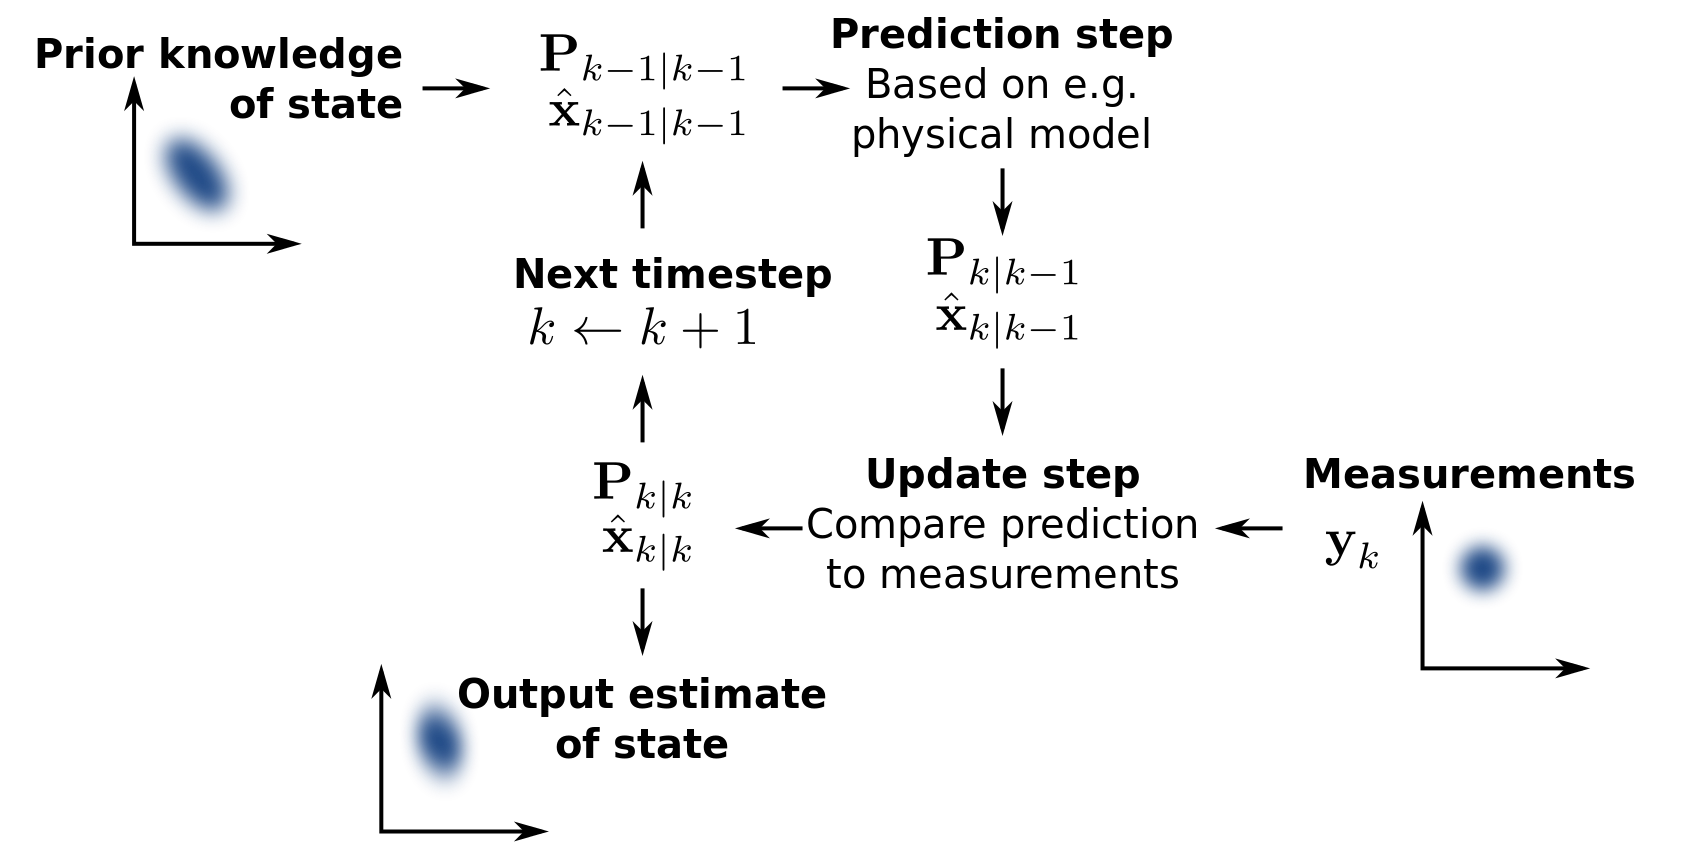
\includegraphics[scale = 0.2]{Images/kf/basic_sch.png}
    \caption[]{Kalman Filter two-step process.\textit{Font: Wikipedia}.}
    \label{fig:kf_sch}
\end{figure}%
The Kalman filter deals really well with uncertainty, it is able to reduce the sensor noise and process noise by the means of making the best guess in the estimate. The statistical algorithm has the property to be a recursive estimator, so it is only needed the previous state and the current measurement to predict the current state.
% Kalman filter prediction always, not only when we dont see the ball!!!!!

The state chosen in our system is considering the motion of the ball as shows eq.\ref{eq:kf_state}.

\begin{align}
    \mathrm{x_k} &= \begin{bmatrix}
           x, y, z, v_x, v_y, v_z, a_x, a_y, a_z
         \end{bmatrix}
    \label{eq:kf_state}
  \end{align}
The process and measurement covariances matrices should be defined In order to initialize the Kalman Filter. These matrices indicates the noise level in the measurement sensors (usually specified by the manufacturer) denoted as R and the noise in the process which is related to the noise in the state denoted as Q. For further information on the calculations for prediction and update steps see section \ref{sec:annex}.




\section{Implementation}
\label{sec:ros}

In this section, we will describe the practical implementation of the algorithms we used to solve the problem. Using ROS requires accommodating the architecture of the application to its protocols and conventions, so we will start by explaining the structure and communication design of our solution. 

\subsection{ROS system design: architecture and communications}

Due to the complexity of the application, we have organized the code in packages according to their functionality area, splitting it into several nodes within each package as well. To make them communicate with each other, it is sort of a convention to use the \textit{publisher-subscriber} system for messages broadcast in continuous streams, such as sensor data or boolean results (like detection). On the other hand, to handle direct communications with the robot, like configuration values, it is better to use services, which allow handling movements on request much more easily. Therefore, all the vision part, and the collision detection in the path planner, were implemented as a network of publishing and subscribing nodes, while the path execution part was coded using the CAROS Service Call Interface for the UR robot. The following list enumerates all the packages in the application.

\begin{itemize}
    \item Packages given at lectures:
        \begin{itemize}
            \item \textbf{CAROS}
            \item \textbf{Point Grey Camera Driver.}
        \end{itemize}
    \item Packages developed during the project:
        \begin{itemize}
            \item \textbf{Planner package.} Contents the following nodes:
                \begin{itemize}
                    \item Collision detector.
                    \item Online planner.
                    \item Other test programs to verify that certain parts are working correctly.
                \end{itemize}
            \item \textbf{Red Ball Detection package.} Contains the following nodes:
                \begin{itemize}
                    \item Right and left image detectors (by color segmentation).
                    \item Kalman filter for obstacle tracking.
                    \item Stereo 3D triangulation.
                \end{itemize}
            \item \textbf{Robot State Monitoring package.} Contains the following nodes:
                \begin{itemize}
                    \item Robot State Monitoring node (displays robot's state variables live).
                \end{itemize}
        \end{itemize}
\end{itemize}

Figure \ref{fig:nodes} shows in a graph the structure of the network. The camera driver runs and broadcast left and right images separately. Then, two independent image detectors are launched, segment the image by colors in the HSV space and detect the approximate coordinates of the center of the ball and publish it in a topic to which the triangulation node is subscribed. Both detectors are synchronized to send 2D coordinates detected at the same point in time. This is done using an internal ROS function called \textit{message\_filters::TimeSynchronizer}, called in the triangulation node itself. If the ball disappears from one of the two images, the system stops triangulating until it is back on both again. Then after calculated the 3D position of the ball in the scene, the triangulation node exports the XYZ coordinates into another topic to which the Kalman node is subscribed.  

\begin{figure}[ht!]
    \centering
    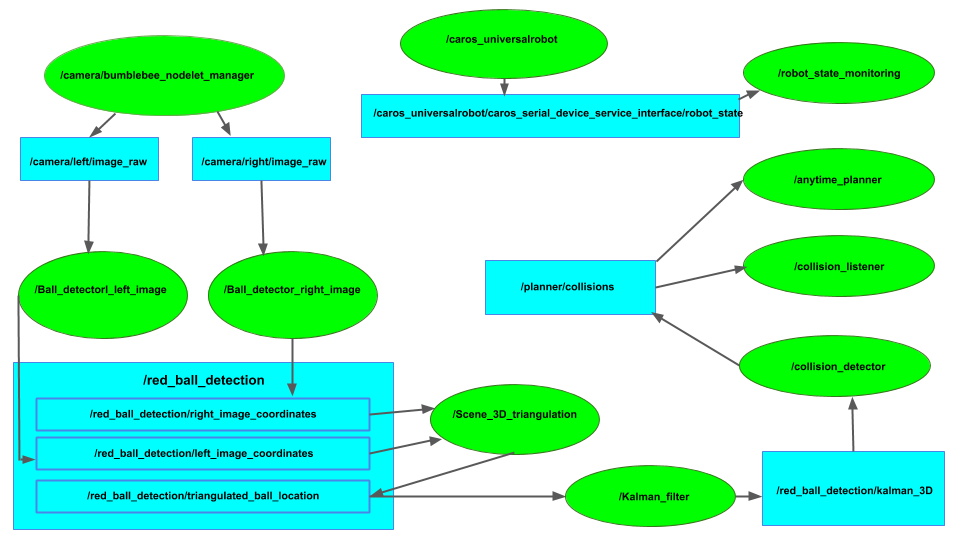
\includegraphics[width=1.1\textwidth]{Images/nodes.png}
    \caption{ROS network. Green ellipses represent nodes whereas blue rectangles represent topics.}
    \label{fig:nodes}
\end{figure}

On the planner side, the first input to the network is the 3D location of the ball tracked in the Kalman node. Until now, all the communications are done using the message type \textit{geometry\_msgs::PointStamped}, which belongs to ROS' API. The collision detector subscribes to the kalman node and uses these three coordinates to update the position of the obstacle and search for potential collisions inside the path calculated and posted by the robot. The collision detector produces boolean messages of the type \textit{std\_msgs::Bool} (also in ROS' API) read by the path planner. While there are no collisions in the path, the robot sticks to the initial plan that was calculated. However, when collisions are detected, the robot stops and replans a new alternative path to reach the goal.

\begin{figure}[ht!]
    \centering
    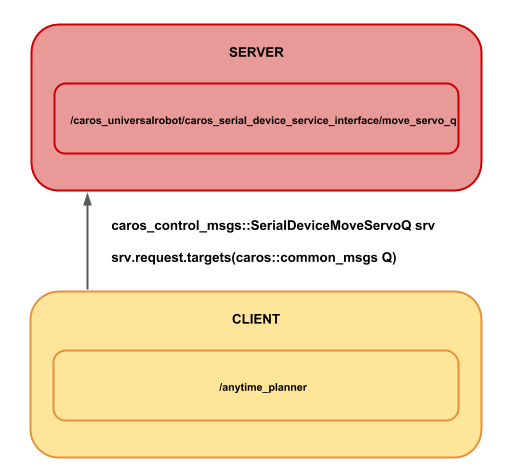
\includegraphics[width=0.6\textwidth]{Images/services.png}
    \caption{CAROS service interface to move the robot by sending Q configuration vectors.}
    \label{fig:services}
\end{figure}

Figure \ref{fig:services} represents the client-server structure of the CAROS serial interface. The planner acts as a client of the \textit{'/move\_servo\_q'} service. When it wants to execute a motion, sends a request with the Q configuration vector that the robot has to reach to the server, which interfaces with the UR controller. 

Now that the flow diagram has been explained, in the next subsections we will explain more in deep how the different nodes were implemented, starting by the vision side.

\subsection{Implementation of the Vision block}

The input to this block are the images that the camera is sending in the ROS network over the topics \textit{'/camera/right/image\_raw'} and \textit{'/camera/left/image\_raw'}. This images correspond to the direct input to the stereo camera, without any type of pre-processing or modification. To be able to use the images, we implemented a bridge between ROS image message type and OpenCV \textit{cv::Mat} image data structure. This operation is done using a function in the ROS API called \textit{cv\_bridge} that easily performs this conversion. With the image converted to \textit{cv::Mat} data type, we applied all the detection techniques to recognize the red ball in the images. Finally, the desired outputs are converted in the last step to the required ROS message types to be exported to other nodes in publishing-subscribing fashion.\\

The code for the vision block was structured in shared libraries in which classes for each separated problem were created: The \textit{'ObstacleDetection'} class to detect the red ball, the \textit{'Stereopsis'} class to perform 3D triangulation and the \textit{'Kalman'} class to track the obstacle in 3D space.

\subsubsection{Ball detection by color segmentation}

The detection function, as well as the subroutine that calls the \textit{cv\_bridge}, is implemented in the \textit{ObstacleDetction.cpp} shared library. Detection is performed individually on the two stereo images, so there are two nodes running the algorithm. These nodes start by calling ROS' \textit{image\_transport} to create subscribers to the \textit{'/image\_raw'} topics. When these images are received, they are converted to \textit{cv::Mat} type and processed. \\

The initial processing steps are Gaussian blurred with a kernel of size 3x3 and converted from BGR to HSV color space. This HSV image is thresholded two times to isolate red colors. The typical range of Hue values for the red is between 160 and 179. Additionally, another threshold is set between 0-10 Hue values to prevent from dark red colors (like maroon or garnet), that could be caused by shadows influencing in the red ball. The two thresholded matrices are combined into one to produce a final binary image.\\ 

The next step is removing noise, in the form of white small dots or shapes apart from the ball, in the binary. To do that, a morphology opening function, with elliptic kernel of size 5, is passed on the image. \\

Finally, to get the center point of the ball, the detector calls the OpenCV function \textit{findContours()}, to get the contour of the ball, and \textit{minEnclosingCircle()} to approximate the minimum circle that covers all the ball area. This last function returns both the center point and the radius of that circle. The last step is to convert the center's pixel coordinates from OpenCV type \textit{$vector<Point2f>$} into \textit{geometry\_msgs::PointStamped}  ROS'  message format to publish them into the topics \textit{'/red\_ball\_detection/right\_image\_coordinates'} and \textit{'/red\_ball\_detection/left\_image\_coordinates'}. \\

\subsubsection{Stereo triangulation}

Stereo triangulation functions are implemented in \textit{Stereopsis.cpp} shared library. The camera intrinsic and extrinsic parameters were estimated during the system's calibration and stored into a \textit{.txt} file that is used by the triangulation node. The first step is to create the projection matrix. Since neither the camera nor the robot base will move from their positions, this matrix is constant all the time. Therefore it is calculated right when the node is run, before it connects to the ROS network of messages. \\

To calculate this projection matrix, as we did in the lectures, two structures were created to store the calibration parameters. The \textit{camera} structure, which stores all the parameters from the calibration \textit{.txt} file, and the \textit{stereoPair} structure, which stores two cameras. This construction is done by the functions \textit{loadCamFromStream()} and \textit{readStereoCameraFile()}. We used the solution provided for the exercise of the second vision lecture of the RoVi2 course \cite{stereopsisExerciseSolution}. \\

With the parameters, function \textit{constructProjectionMat()} constructs a projection matrix as explained in section \ref{sec:tri}, both stored in the \textit{camera} structure.\\

With this matrix already built, the triangulation node subscribes to the detection topics. It is required to have this communication synchronized, to receive coordinates that were detected in both images at the same time. Therefore, the subscribers are not created with the normal procedure, but with the \textit{message\_filters::Subscriber} class. The \textit{Message Filters} library (ROS API) allows managing many messages at once, filtering them by some property. For time synchronization, we use the \textit{timeStamp}. In that way, the triangulation node, when it calls the callback function to process the information coming from the detectors, only uses those messages that come with the same \textit{timeStamp.} As we mentioned above, this synchronization is done using another \textit{message\_filters} function: \textit{message\_filters::TimeSynchronizer}. \\

When the node has already the coordinates of the ball in both images, it performs triangulation using the OpenCV function \textit{triangulatePoints()}, called inside \textit{Stereopsis::calculate\_3D\_location()}, which uses both left and right camera projection matrices and detected points as inputs. It produces a vector that contains the XYZ coordinates of the ball in the real world, with respect to the robot base and in mm. \\

This vector is, finally, transformed again into \textit{geometry\_msgs::PointStamped} message format and published into the topic \textit{'/red\_ball\_detection/kalman\_3D'}. It is important to also synchronize the output message with the inputs. This is done just by coping the \textit{timeStamp} header of the input messages into the output one.

\subsubsection{Kalman filter}

There are three files related to the implementation of the filter:\textit{kalman\_3d.h}, \textit{kalman\_3d.cpp} and \textit{kalman\_ros.cpp}. The firsts files is to create a Kalman Filter class which will contain the methods required to calculate the best estimate point of the ball center. The last one \textit{kalman\_ros.cpp} enables the ROS interface subscriber/publisher to receive and send messages from the \textit{triangulation} to the \textit{collision\_detector} nodes.

In order to implement the algorithm it is used \textit{OpenCV} libraries and \textit(kalman\_template.cpp) provided by the lectures of the course. It is needed to describe the state of the ball that the Kalman Filter will track. In this case is possible to define the state vector as only the position of the ball or adding features such as the velocity and the acceleration of the ball in order to make the estimation more accurate. For this project it is considered the position, velocity and acceleration in the space X,Y and Z as a state vector (see eq. \ref{eq:kf_state} in section \ref{sec:kal}). Furthermore, is needed to describe how many measurements have as input the filter which is the position of the ball's center in the space. Once this is described the Kalman filter is created by \textit{OpenCV} function. However, it is needed to describe a few matrices such as, the transition matrix, which is the relation between the measurements and the state vector. This matrix determines the kinetic equations  by calculating the first and second order derivatives respect to the position of the ball. Additionally, it is required to initialize the covariances matrices of the measurement and process. Which determines the noise level in the process and in the sensors for calculating the best estimate.

Once the initialization is done, the two functions \textit{KALMAN::predict} and
\textit{KALMAN::correct} describes the two-step process mentioned on section \ref{sec:kal}. These functions are called continously in order to predict the position of the ball and correct it based on the measurement received. These two functions are called in another method (\textit{KALMAN::Kalman\_filter\_3D}) which will contain the two-step process along as a \textit{SkipcCorrection} in the case that the ball is missing and the Kalman Filter only needs to predict the state of the object.

Finally, the function \textit{KALMAN::ball\_location\_kf\_callback} which is subscribed to the triangulation node and calls the Kalman function and finally publish te position of the ball in the space.

%explain callback function for the process of receiveing and sending msgs through ros nodes


\subsection{Implementation of the Planner block}
% Talk the WorkCell approach, move the ball, the collision detector... leave the planning function for the end.
In the robotics part there are two main important nodes: the \textit{anytime\_planner} and the \textit{collision\_detector}. This nodes depend not only in the network but also in the RobWorkStudio simulated WorkCell, which contains all the geometries present in the scene (table, computer, ball, robot...). The idea is that to check for collisions, the scene in the WorkCell is updated with the 3D ball coordinates and the robot is moved to see if states in the path collide at some point with the ball or not. Therefore, the simulated scene is updated with the real world information coming from the sensors all the time as well. This bridge between the WorkCell and the robot's actual space is extremely important for the system. \\

To add the geometry of the red ball into it, we created a CAD model of it into the \textit{.xml}, setting the radius and creating it as a movable frame. Then, in the code function that opens and loads the WorkCell into the program, the ball is cast into a movable frame as well, that is able to move it around to with the input coordinates coming from the communication with the Kalman node. The setup of the WorkCell is shown in figures \ref{fig:wc1} and \ref{fig:wc2}. It is worth mentioning that the ball's CAD model is actually bigger than the real ball, considering some clearance for the system to avoid collisions securely. \\

\begin{figure}[ht!]
\centering
\begin{minipage}{.5\textwidth}
  \centering
  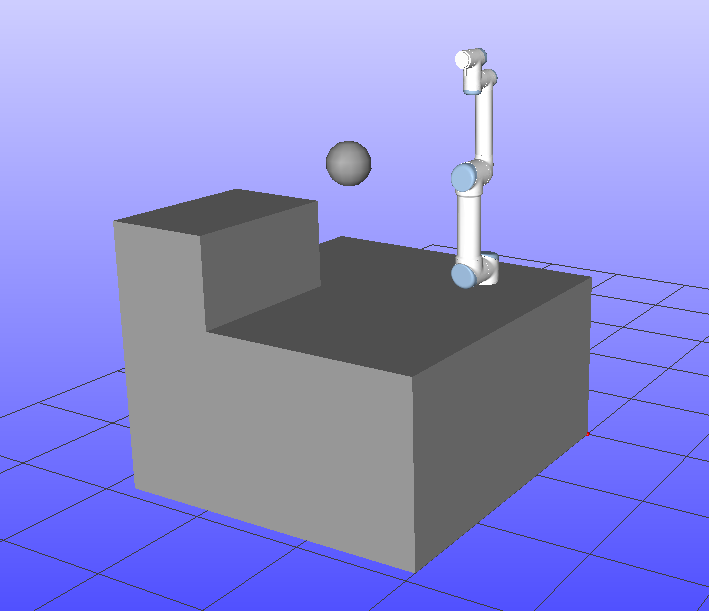
\includegraphics[width=.8\linewidth]{Images/wc1.png}
  \captionof{figure}{Capture from RobWorStudio of the WorkCell setup.}
  \label{fig:wc1}
\end{minipage}%
\begin{minipage}{.5\textwidth}
  \centering
  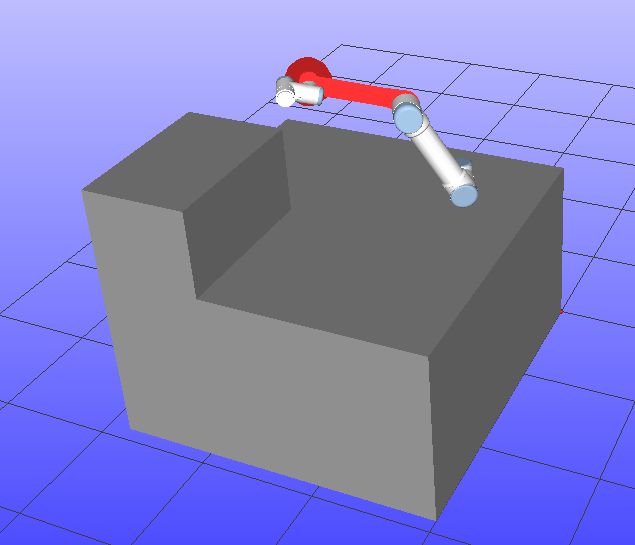
\includegraphics[width=.8\linewidth]{Images/wc2.png}
  \captionof{figure}{Capture of the robot and the ball colliding.}
  \label{fig:wc2}
\end{minipage}
\end{figure}

The subroutine that elaborates search for collisions in the path is not implemented in the planner, but in a separate node. To share the paths that the planner calculates, each time it saves the plan data into a text file that is opened and read cyclically by the collision detection node.\\

The implementation of this part followed the same methodology as in the vision part, creating shared libraries with classes for different scopes. 

\subsubsection{Collision Detector}
% Talk about why we use the plan.txt instead of trajectory.txt to detect collisions
The collision detector is mainly implemented in the class \textit{AnytimePlanning}. This node is subscribed to the topic in which the Kalman node broadcasts the location of the ball. It also reads constantly the paths that the planner calculates from the file were they are being saved and updated.\\

It uses the coordinates of the ball to move the red ball around the scene inside the WorkCell. This is done in using several functions. The first one, \textit{move\_red\_bal()} transforms the coordinates given in \textit{geometry\_msgs::PointStamped} into meters (RobWork's default unit). Then, it moves the ball by using those coordinates to set a new transform matrix for the red ball's movable frame. After moving it, the function \textit{sphere\_strategy()} creates a new collision strategy based on the WorkCell and the ball's location. The last step is to use this strategy to run a \textit{checkCollisions()} functions over the path. We implemented the collision checker to check the path with a reasonably high resolution, not only in the nodes but between them as well. The result of this \textit{checkCollisions()} function is a boolean variable, which is published in the topic \textit{'/planne/collisions'} using the message format \textit{std\_msgs::Bool}. \\

One thing to remark is that, the collision detector can both examine the raw plan calculated by the path planning algorithm, or it can evaluate the trajectory that is later interpolated around this path. This trajectories are generated with time-spaces of 0.05 seconds between consecutive Q vectors. Since the tolerances in the simulated WorkCell are big, and the robot's diameter of its several parts is bigger than in reality, sometimes evaluating the trajectory reports errors. This mistakes are caused by the tolerance issue, which reports that in the simulated WorkCell, self-collisions are detect between robot parts are detected due to the small displacement (0.05 seconds) carried from one node to the next. \\

To overcome this problem, the \textit{plan.txt} file, which contains the raw path prior to be interpolated, is used. This provides enough distance between two consecutive Q vectors to avoid erroneous self-collisions. At the same time, it does not compromise the task by missing collisions, because the nodes in the path are not far enough from each other for that (this last issue, clearly depends on the epsilon parameter of the RRT algorithm). 

\subsubsection{Online planner}
The online path planner node subscribes to the topic published by the collision checker, calculates collision-free paths and works as a client of Caros in order to move the robot. The main idea is to feed the starting and goal configurations to the planner, which calculates a collision-free path and writes it to a file which is read by the collision checker. Whenever the ball is moved in the workcell and a collision appears in the already calculated path, the collision checker publishes the collision status variable accordingly. The path planner node, while iterating from node to node of the path and sending them to the robot, is always listening to the collision status and replans if necessary. After every replanning, a trajectory is interpolated. To send the trajectory to the robot, the state of the robot is constantly monitored. If the state is close enough to the actual node the reach, only then we send the new node of the path. For this purpose, an Euclidian-distance function was implemented.
\newpage
\section{Experiments and Evaluation}

\subsection{Evaluation of the detection node.}

For the whole system to succeed, it is extremely important that the image detection algorithm is robust and with high accuracy rates. To evaluate its performance, the detector was tested on a video sequence such as the one shown in figure \ref{fig:feature_extraction}, achieving almost 100\% of accuracy detecting the ball in working conditions. However, we discovered that shadows can make the detector unreliable. Furthermore, having multiple red objects in the scene will result in a fail.

\subsection{Evaluation of the triangulation node.}

The triangulation node was evaluated with a test program which received the messages and transform it to robot base coordinates. In that way, moving the obstacle along the XYZ axes of the robot's base frame, it could be checked on the program if the X, Y, and Z coordinates were correctly assigned.

\subsection{Evaluation of the Kalman filter}
Three test are designed in order to evaluate the functionality and performance of the 3D Kalman Filter. As the objective is to track the ball.

We elaborated a first test based on motion tracking, where the ball is missing for a period of time and the statistical algorithm is able to predict the position of the ball . 
The second test is designed to determine which values for the process and measurement covariances matrices are needed for a good performance of the filter. Lastly, a third test that will prove how the Kalman Filter behaves with a miss recognition of the ball.
\newpage
\subsubsection{Test 1: Motion tracking}
The Kalman filter state considers the position, velocity, and acceleration of the ball. This allows the filter to learn the motion of the ball. So if we expect to loss the ball in a trajectory, the statistical algorithm will predict the next states of the ball based on the motion of the lasts measurements it got. In a practical point of view, the Kalman filter is able to remember the linear motion that the ball had, so if we are moving the ball linearly it will consider that motion and predict based on that. Non-linearities when the ball is missing would be not considered by the algorithm.

The test is quite simple, first of all we put the ball in one corner of the camera range and we start moving smoothly the ball by using a stick. The movement is a linear movement, but suddenly the ball passes behind the robot without being in camera range. It can be observed in the red line of the fig. \ref{fig:kf_motion} that the measurements are gone in that moment. However, the Kalman filter is able to predict the linear trajectory and in the end when the ball is in the camera range the Kalman Filter corrects its states.
%\vspace{3 pt}
\begin{figure}[ht!]
    \centering
    \captionsetup{justification=centering,margin=1cm}
    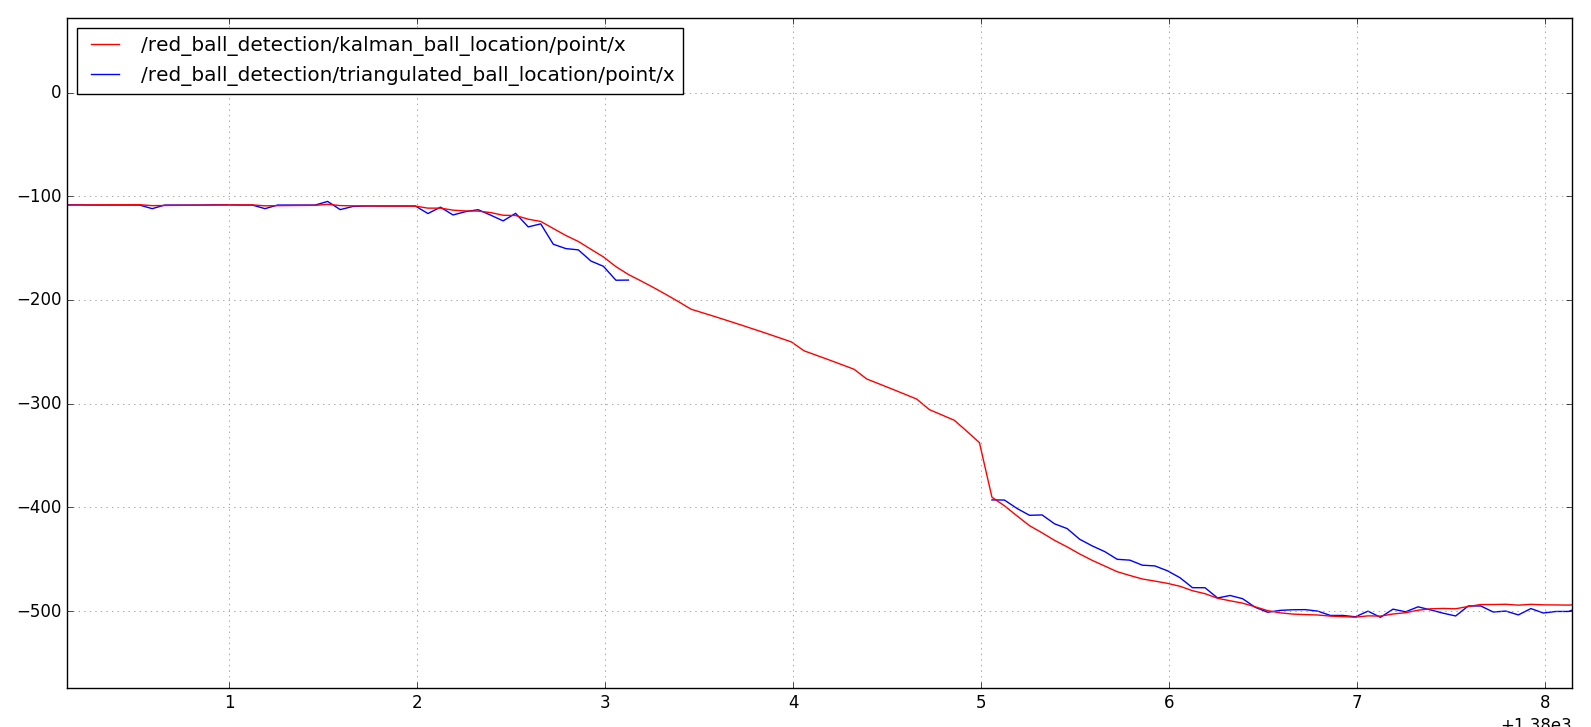
\includegraphics[scale = 0.30]{Images/kf/motion_tracking.png}
    \caption[]{Kalman Filter motion tracking.}
    \label{fig:kf_motion}
\end{figure}%

% PLOT!
% lets make a test moving the ball continously with a low-noise R and Q to see what happens, it will show a sinousoid??? KF is linear!! :S
\newpage
\subsubsection{Test 2: Uncertainty in Kalman Filter}

The second test consist in moving the ball continuously in 'x' axis for different noise levels in measurement and process covariances matrices. The purpose is to see how the filter adapts itself in the motion described. Moreover, it is expected to determine which values are suitable for our application. In fact, we want to determine the motion that the \textit{Kalman Filter} should track. Moreover, we need to know how fast is the ball suppose to move. Faster motions than expected should be filtered.

The motion that defines the limit where the filter should act is found empirically. The ball is moved from two states in 'x' direction with the motion we should remove. In fig. \ref{fig:kf_uncertainty} left side is noticeable how the Kalman Filter adapts to the motion completely. The motion applied to the ball is quite fast, so a miss detection of the ball in a remote place on the workcell would lead to a bad tracking of the ball. In the right side of the image is observed that the output of the Kalman Filter is a bit smooth compared with the previous image. In this case, the statistical algorithm with high-level noise is more robust to out-layers rather than the previous performance of the filter.
\begin{figure}[ht!]
\centering
\captionsetup{justification=centering,margin=1cm}
\resizebox{\textwidth}{!}{\begin{tabular}{cc}
%\hline
\subf{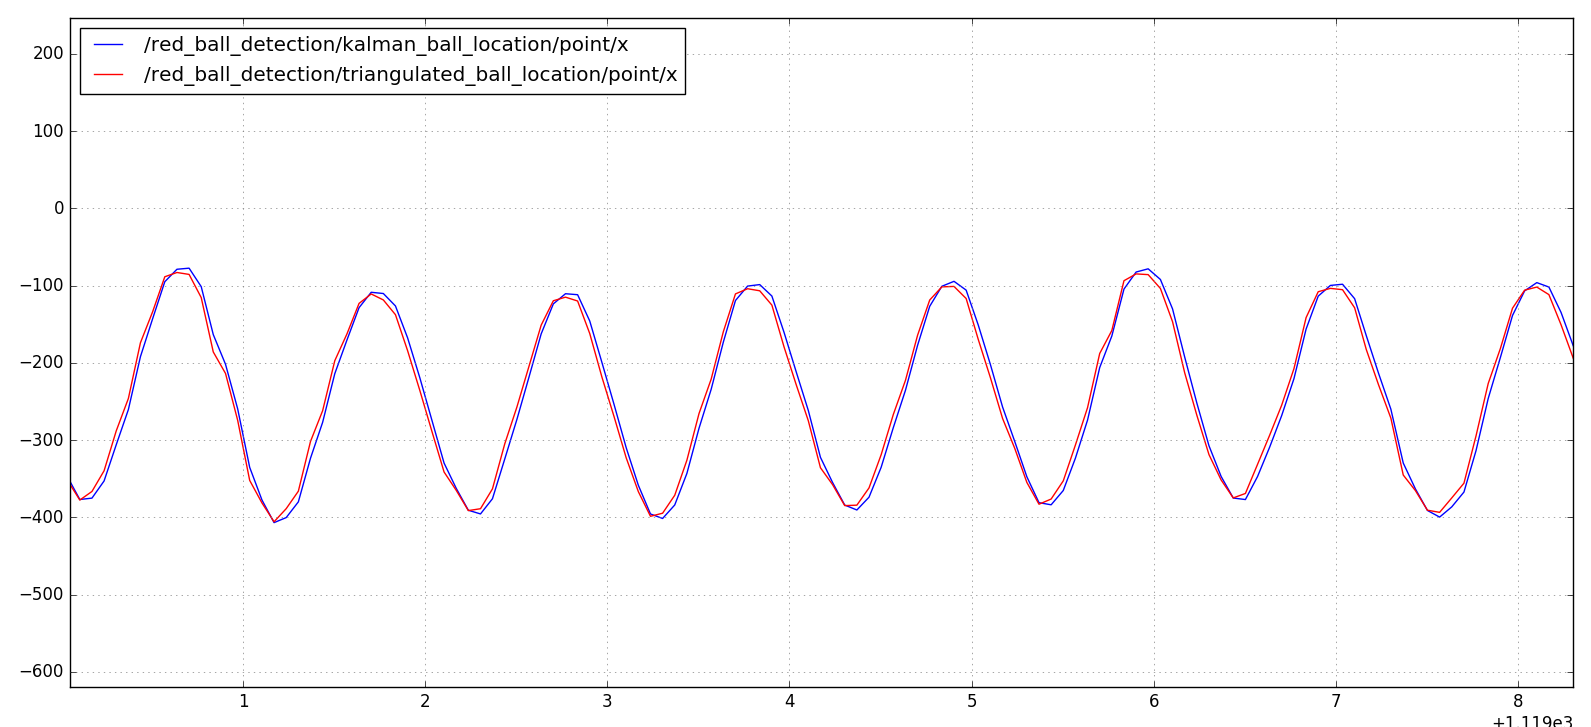
\includegraphics[width=60mm,height=60mm]{Images/kf/noise_0p1.png}}
     {Kalman filter R and Q with 0.1}
&
\subf{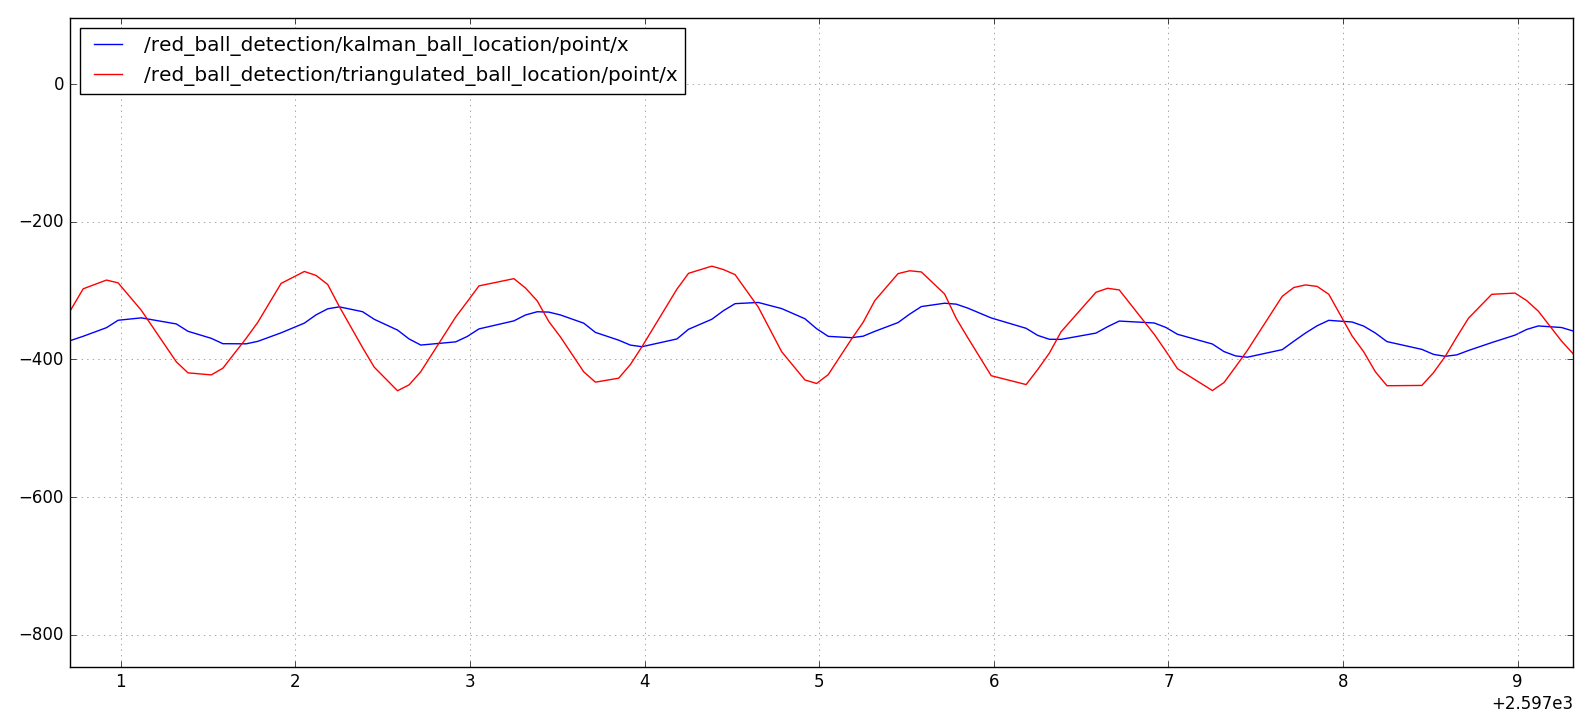
\includegraphics[width=60mm,height=60mm]{Images/kf/noise_150.png}}
     {Kalman filter R: 150 and Q: 0.1}
%\hline
\end{tabular}}
\caption{Uncertainty in measurement.}
\label{fig:kf_uncertainty}
\end{figure}  
   
\newpage
\subsubsection{Test 3: Miss recognition}

The third test consist to reproduce a miss recognition of the ball's position. For doing that, we grab the ball with our hand covered by black clothes and do a really fast movement of the ball in axis 'x'. 

Using the same levels of noise as before. It is found something interesting, the filter with low-noise levels is almost adapted by one measurement. The differential position is about 30 cm, which makes the Kalman Filter a really fast approach to a motion that moves 30 cm per measurement. However, this performance does not fit very well to our system specifications. A movement with those characteristics should be filtered. In the right-side of the figure and with a high level noise in covariances matrices the filter performs really well in our own specifications because it does not adapt that good to the motion specified, but in fact it starts to do it. So we expect to adapt completely in 3-4 measurements. 

In this case, the main key point is to define the expectation of a miss recognition. For this project it is considered around 3-4 measurements a valid move of the ball, mainly because, the motion is not clearly defined. The ball is moved with a stick which makes the system quite impredecible and the Kalman Filter needs to track the ball for those movements. 
% In order to reduce the complexity the movement of the ball could be linear defined so the ball is able to track it. Or an extended Kalman filter or unscented Kalman filter can be applied
\begin{figure}[ht!]
\centering
\captionsetup{justification=centering,margin=1cm}
\resizebox{\textwidth}{!}{\begin{tabular}{cc}
%\hline
\subf{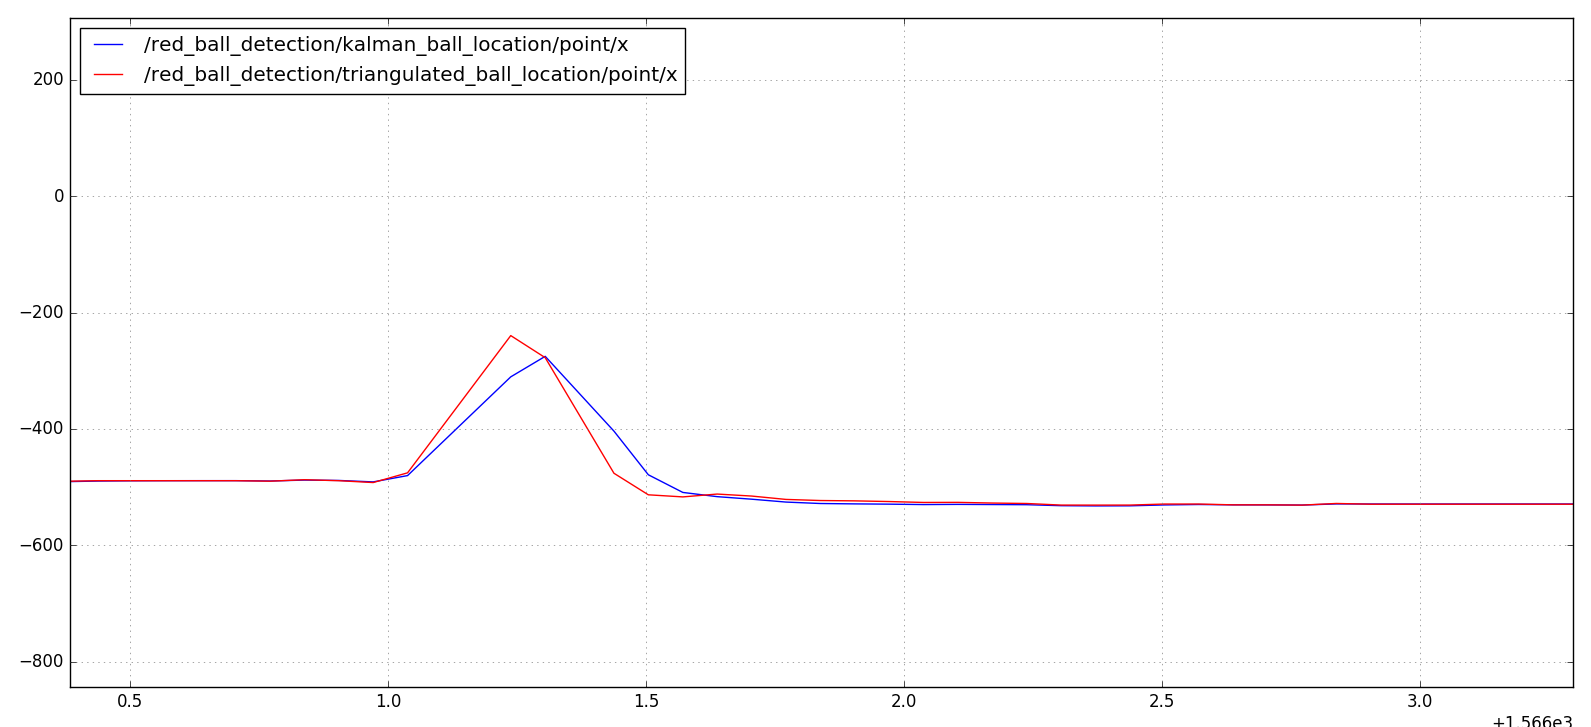
\includegraphics[width=60mm,height=60mm]{Images/kf/misrecognition_noise0p1.png}}
     {Kalman filter low-noise levels}
&
\subf{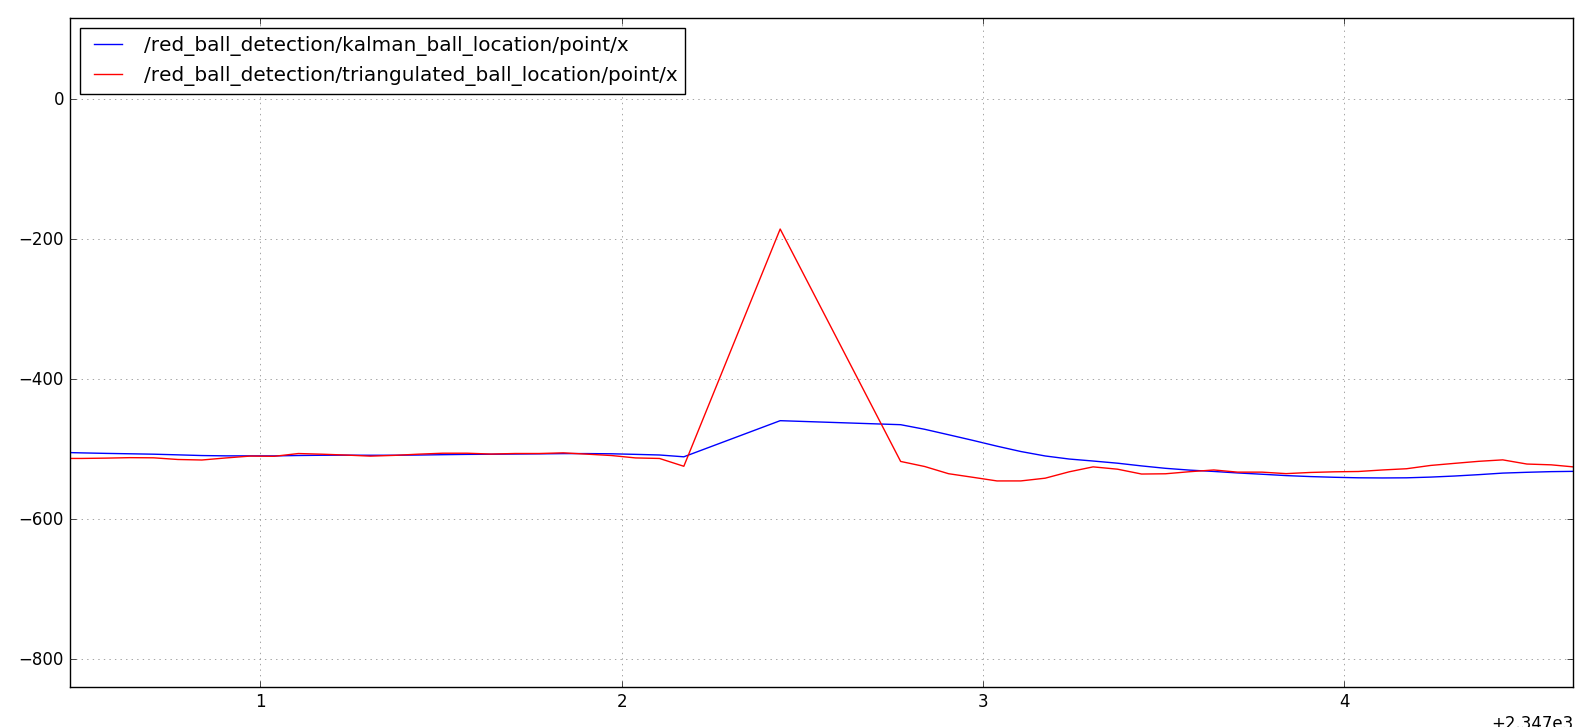
\includegraphics[width=60mm,height=60mm]{Images/kf/misrecognition_noise150.png}}
     {Kalman filter high noise}
%\hline
\end{tabular}}
\caption{Miss recognition in measurement.}
\label{fig:kf_uncertainty}
\end{figure}  
\section{Results}

In this sections is exposed the performance of the algorithms which this project focuses on: The RRT* planner for the robotics side and the Kalman filter for the vision side.

In order to evaluate the Kalman Filter: the computation time, error response for different noise levels. The execution time of the statistical algorithm is \textbf{51 $\mu$s} which makes sense due the fact that this algorithm is used for applications where the computational time is required to be low.

In order to see how the different noise levels in the process and measurement covariance matrices affects the performance of the Kalman filter. It is decided to choose between high and low values and switch the combinations to see how is the error in motion tracking. The empirical tests has been done in static and dynamic environments.
\begin{figure}[ht!]
\begin{subfigure}{.5\textwidth}
  \centering
  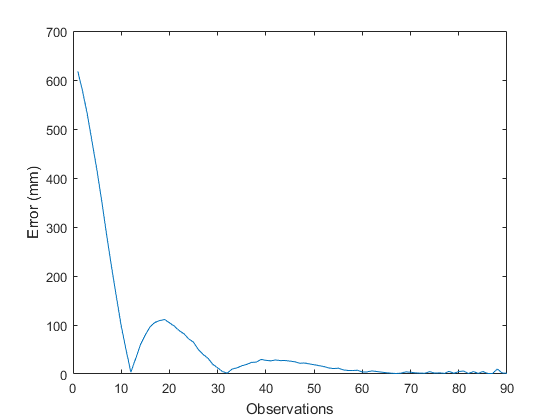
\includegraphics[width=.8\linewidth]{Images/kalman_plots/static_1.png}
  \caption{Static-1: Q = 0.01 and R = 1}
  \label{fig:sfig1}
\end{subfigure}
\begin{subfigure}{.5\textwidth}
  \centering
  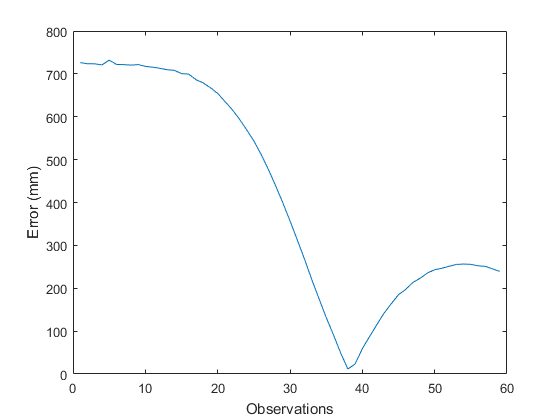
\includegraphics[width=.8\linewidth]{Images/kalman_plots/static_2.png}
  \caption{Static-2: Q = 0.01 and R = 100}
  \label{fig:sfig2}
\end{subfigure}
\begin{subfigure}{.5\textwidth}
  \centering
  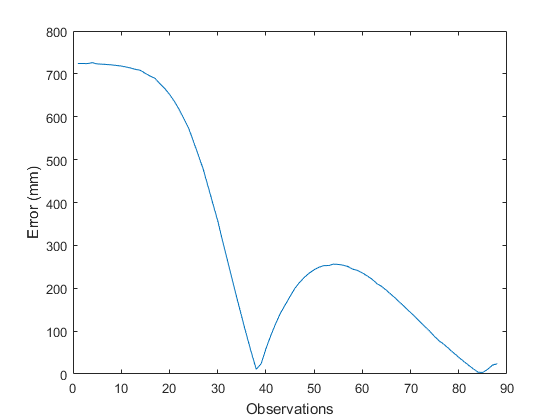
\includegraphics[width=.8\linewidth]{Images/kalman_plots/static_3.png}
  \caption{Static-3: Q = 200 and R = 0.1}
  \label{fig:sfig3}
\end{subfigure}
\begin{subfigure}{.5\textwidth}
  \centering
  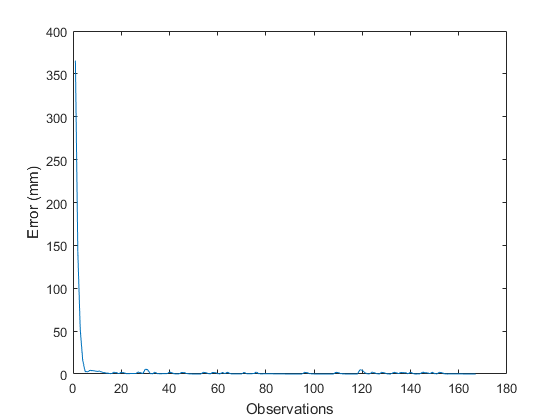
\includegraphics[width=.8\linewidth]{Images/kalman_plots/static_4.png}
  \caption{Static-4: Q = 300 and R = 300}
  \label{fig:sfig4}
\end{subfigure}
\caption{Error plots of the Kalman filter and measurement in static.}
\label{fig:static_kalman}
\end{figure}

To check the error of the Kalman Filter in dynamic environment see section \ref{sec:annex}.
\newpage
To evaluate the anytime dynamic path planner performance, we investigated run-time of the collision checker algorithm against the resolution. We used pruned paths from the initial to the end configuration each time and performed collision checking 20, 50 and 500 configurations between each node.

50 measurements where taken at each level and the averages are shown in Table \ref{tab:coll}.
\begin{table}[ht!
]
\centering
\label{plan:accuracy_table}
    \begin{tabular}{|c|c|}
    \hline
    Nº Nodes & Time(s))  \\ \hline
      108       &  0.195     \\ \hline
      243      & 0.21      \\ \hline
        2561      &  0.38       \\ \hline
    \end{tabular}
    \caption[]{\textit{ Collision performance.}}
    \label{tab:coll}
\end{table}

We measured the runtime of the planner from the initial configuration to the final one. We investigated the number of nodes generated and the resulting path after pruning. We took 50 measurements at each level of the extend parameters and we plot the averages in Table \ref{tab:plan}

\begin{table}[H]
\centering
\label{plan:accuracy_table}
    \begin{tabular}{|c|c|c|c|}
    \hline
    Extend ($\epsilon$)  & Nº Nodes & Nº Nodes (opt.) & Planner time(s)  \\ \hline
    0.05          &  193  & 6 &  0.47   \\ \hline
    0.2              &  51 & 5 & 0.070    \\ \hline
    0.5          & 24 & 4 & 0.026   \\ \hline
    2          &  6 & 3 & 0.007      \\ \hline

    \end{tabular}
    \caption[]{\textit{RRT*} performance.}
    \label{tab:plan}
\end{table}


\newpage
\section{Discussion}
\label{sec:dis}
%2D vs 3D Kalman filter
We had some discussions about in which dimensionality the Kalman filter should be implemented. In theory, the filter should be able to work well in both cases. However, implementing a 2D Kalman filter would imply initialize two filters where the process and measurement noises would be different. Moreover a synchronization of them along with the object recognition could be required. In order to implement into the system is a bit complex rather than in the space. The main drawback of this choice is that we were not able to show the Kalman filter response in the 2D image. It would require extra time that we prefer to spend in another issues.



\section{Conclusion}
\label{sec:con}
We could conclude that the project was successful in a sense that all the components were successfully implemented. In addition to this, we succeeded integrating a complex system using multiple frameworks. The robot managed to perform the object avoidance with a short computation time and a short reaction time to a collision in the path. There are options to improve the individual components of the system, but there is nothing much left to do with the integration of them. We discuss the possibilities for improvements in the next section.

%Each component of the system works, the components are well integrated and the system manages to what it has to. WE MADE IT WORK and we did not just implement separate components but they are actually put together!!
%We have some improvements to do (future work), we need to evaluate, we can make separate components work faster / more accurate, but no big changes have to be made

\section{Future Work}
At this moment, we have several useful features of the Kalman filter, but we also wanted to give the predictions about the expected position of the ball based on the measurements at a given moment to the planner. This functionality would be very useful for object avoidance with a moving object where the planner finds a path without colliding the ball in anytime. 

We could use both the measurement and the prediction as an input to the workcell to define the collision volume in a more sophisticated way. A simple way would be placing the object in both positions. Another way could be connecting the points by sweeping the object in the 3D space from one to the other.

Our observation is that when we try to place the ball in the path of the robot, we often have to move the ball close to the robot. When the robot detects collision in the configuration in which it is at a given moment, it stops and tries to replan, but never succeeds, because the actual configuration is always part of the path. A small modification in the implementation has to be made so that the robot leaves the collision configuration and continues a collision-free path.

Additionally an extension of the Kalman Filter could be implemented for non-linear motions. At this moment, the filter is able to track the ball and predict linear movements. In case that the filter is only predicting and non-linearities come up to the system, it would end up in a bad tracking. Adding an Extended Kalman Filter or Unscented Kalman Filter could help to predict the non-linear trajectories of the ball making a better accurate tracking.

Finally, a more accurate transformation would help a lot to evaluate the system as a whole. We noticed that there is an error in the result of the triangulation which scales with the distance from the camera. Sometimes the robot hit the ball and we were not able to determine if it's the result of a bigger error in the triangulated 3D coordinate.

%Kalman filter prediction
%Defining a collision volume which connects the actual coordinate and the predicted coordinate
%Moving the robot even if it is in collision in the very first node
%Better calibration
\newpage
\setlength{\parskip}{1em}
\section{Annex}
\label{sec:annex}
\subsection{Kalman Filter equations}
Nomenclature provided by \textit{Wikipedia}:

$F_k$: transition matrix

$H_k$: measurement model

$Q_k$: process covariance matrix

$R_k$: measurement covariance matrix

$B_k$: control-input model

$u_k$: control vector

$w_k$: process noise (assumed normally distributed)

\textbf{Equations for prediction step:}

Predicted (a priori) state estimate:

	{\displaystyle {\hat {\mathbf {x} }}_{k\mid k-1}=\mathbf {F} _{k}{\hat {\mathbf {x} }}_{k-1\mid k-1}+\mathbf {B} _{k}\mathbf {u} _{k}} {\displaystyle {\hat {\mathbf {x} }}_{k\mid k-1}=\mathbf {F} _{k}{\hat {\mathbf {x} }}_{k-1\mid k-1}+\mathbf {B} _{k}\mathbf {u} _{k}}
	
Predicted (a priori) estimate covariance:

	{\displaystyle \mathbf {P} _{k\mid k-1}=\mathbf {F} _{k}\mathbf {P} _{k-1\mid k-1}\mathbf {F} _{k}^{\mathrm {T} }+\mathbf {Q} _{k}} {\displaystyle \mathbf {P} _{k\mid k-1}=\mathbf {F} _{k}\mathbf {P} _{k-1\mid k-1}\mathbf {F} _{k}^{\mathrm {T} }+\mathbf {Q} _{k}}
	
\textbf{Equations for update step:}

Innovation measurement

	{\displaystyle {\tilde {\mathbf {y} }}_{k}=\mathbf {z} _{k}-\mathbf {H} _{k}{\hat {\mathbf {x} }}_{k\mid k-1}} {\tilde {\mathbf {y} }}_{k}=\mathbf {z} _{k}-\mathbf {H} _{k}{\hat {\mathbf {x} }}_{k\mid k-1}
	
Innovation covariance

	{\displaystyle \mathbf {S} _{k}=\mathbf {R} _{k}+\mathbf {H} _{k}\mathbf {P} _{k\mid k-1}\mathbf {H} _{k}^{\mathrm {T} }} {\displaystyle \mathbf {S} _{k}=\mathbf {R} _{k}+\mathbf {H} _{k}\mathbf {P} _{k\mid k-1}\mathbf {H} _{k}^{\mathrm {T} }}
	
Optimal Kalman gain

	{\displaystyle \mathbf {K} _{k}=\mathbf {P} _{k\mid k-1}\mathbf {H} _{k}^{\mathrm {T} }\mathbf {S} _{k}^{-1}} {\displaystyle \mathbf {K} _{k}=\mathbf {P} _{k\mid k-1}\mathbf {H} _{k}^{\mathrm {T} }\mathbf {S} _{k}^{-1}}

Updated (a posteriori) state estimate

	{\displaystyle {\hat {\mathbf {x} }}_{k\mid k}={\hat {\mathbf {x} }}_{k\mid k-1}+\mathbf {K} _{k}{\tilde {\mathbf {y} }}_{k}} {\hat {\mathbf {x} }}_{k\mid k}={\hat {\mathbf {x} }}_{k\mid k-1}+\mathbf {K} _{k}{\tilde {\mathbf {y} }}_{k}

Updated (a posteriori) estimate covariance

	{\displaystyle \mathbf {P} _{k|k}=(\mathbf {I} -\mathbf {K} _{k}\mathbf {H} _{k})\mathbf {P} _{k|k-1}(\mathbf {I} -\mathbf {K} _{k}\mathbf {H} _{k})^{T}+\mathbf {K} _{k}\mathbf {R} _{k}\mathbf {K} _{k}^{T}}
	
Measurement residual

	{\displaystyle {\tilde {\mathbf {y} }}_{k\mid k}=\mathbf {z} _{k}-\mathbf {H} _{k}{\hat {\mathbf {x} }}_{k\mid k}} {\displaystyle {\tilde {\mathbf {y} }}_{k\mid k}=\mathbf {z} _{k}-\mathbf {H} _{k}{\hat {\mathbf {x} }}_{k\mid k}}
\newpage
\subsection{Kalman Filter performance for different noise levels}
In the dynamics environment:
\begin{figure}[ht!]
\centering
\captionsetup{justification=centering,margin=1cm}
\resizebox{\textwidth}{!}{\begin{tabular}{cc}
%\hline
\subf{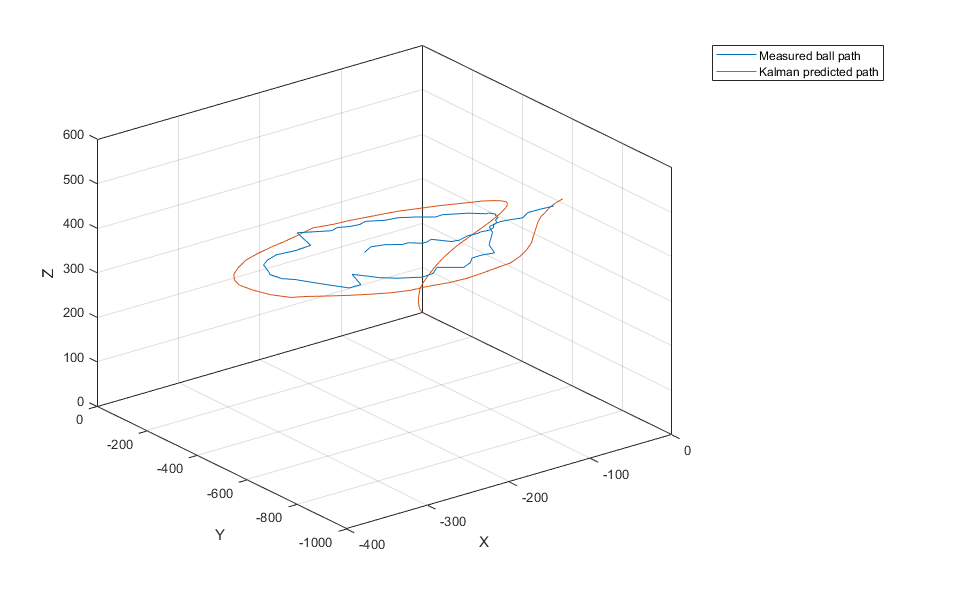
\includegraphics[width=60mm,height=60mm]{Images/kalman_plots/first_dyn_1.png}}
     {KF and Measurements in space.}
&
\subf{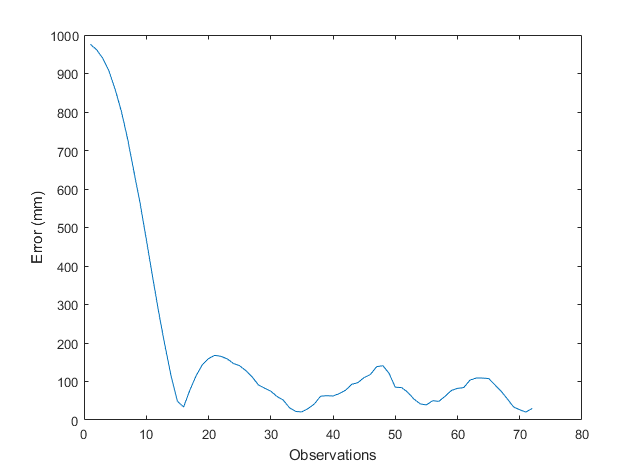
\includegraphics[width=60mm,height=60mm]{Images/kalman_plots/first_dyn_error.png}}
     {Kalman Filter error.}
%\hline
\end{tabular}}
\caption{Dynamic - 1: Q = 0.01 and R = 1.}
\label{fig:kf_dyn1}
\end{figure} 

\begin{figure}[ht!]
\centering
\captionsetup{justification=centering,margin=1cm}
\resizebox{\textwidth}{!}{\begin{tabular}{cc}
%\hline
\subf{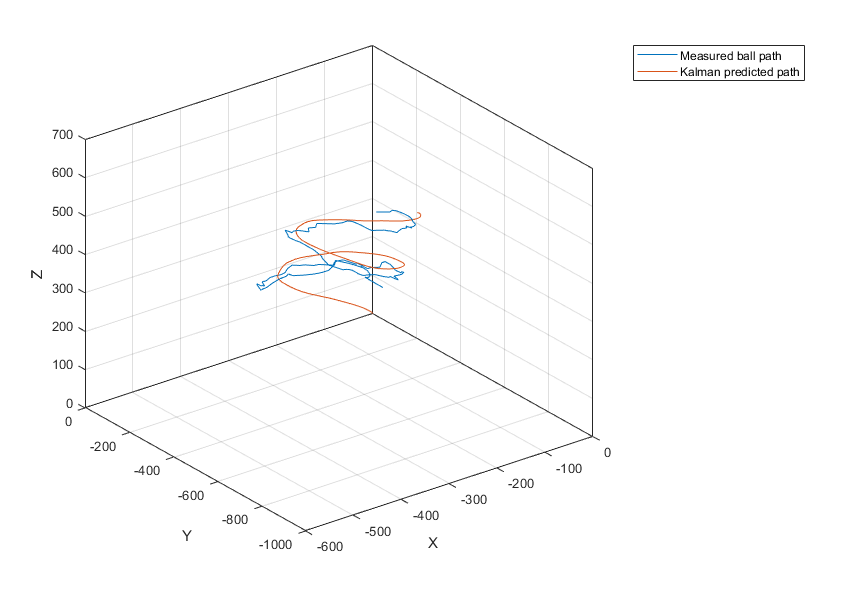
\includegraphics[width=60mm,height=60mm]{Images/kalman_plots/second_dyn_1.png}}
     {KF and Measurements in space.}
&
\subf{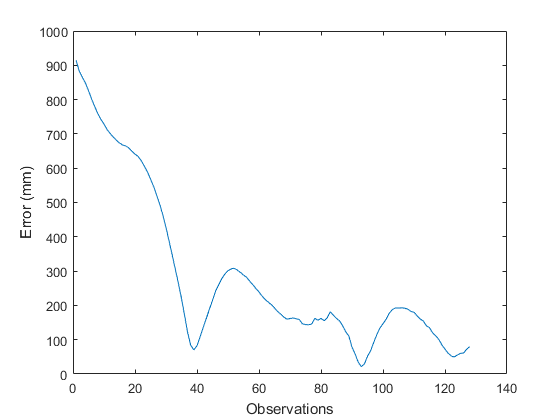
\includegraphics[width=60mm,height=60mm]{Images/kalman_plots/second_dyn_error.png}}
     {Kalman Filter error.}
%\hline
\end{tabular}}
\caption{Dynamic - 2: Q = 0.01 and R = 100}
\label{fig:kf_dyn2}
\end{figure} 

\begin{figure}[ht!]
\centering
\captionsetup{justification=centering,margin=1cm}
\resizebox{\textwidth}{!}{\begin{tabular}{cc}
%\hline
\subf{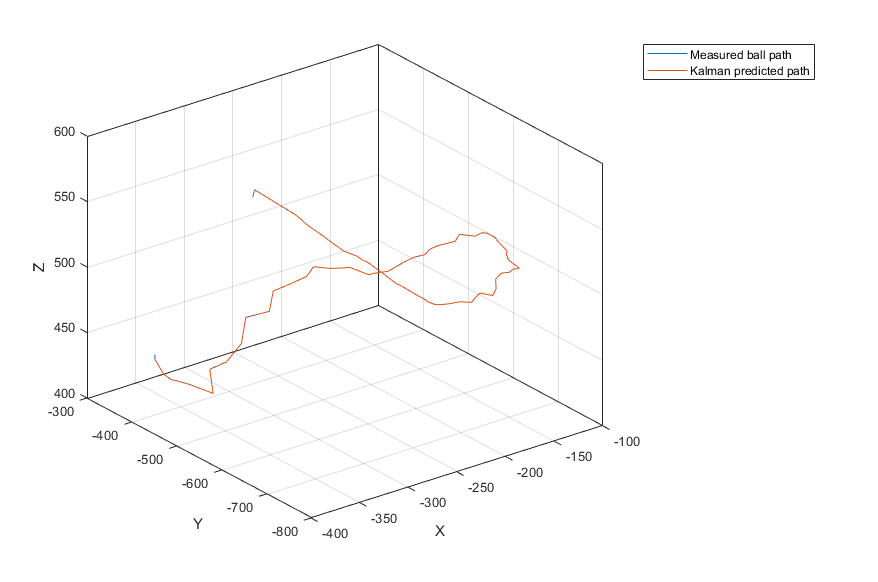
\includegraphics[width=60mm,height=60mm]{Images/kalman_plots/third_dyn_1.png}}
     {KF and Measurements in space.}
&
\subf{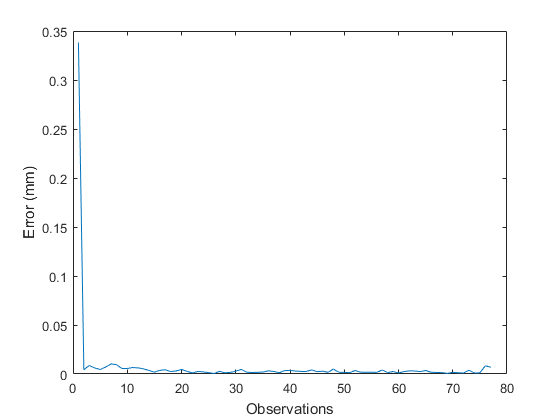
\includegraphics[width=60mm,height=60mm]{Images/kalman_plots/third_dyn_error.png}}
     {Kalman Filter error.}
%\hline
\end{tabular}}
\caption{Dynamic - 3: Q = 200 and R = 0.1}
\label{fig:kf_dyn3}
\end{figure} 

\begin{figure}[ht!]
\centering
\captionsetup{justification=centering,margin=1cm}
\resizebox{\textwidth}{!}{\begin{tabular}{cc}
%\hline
\subf{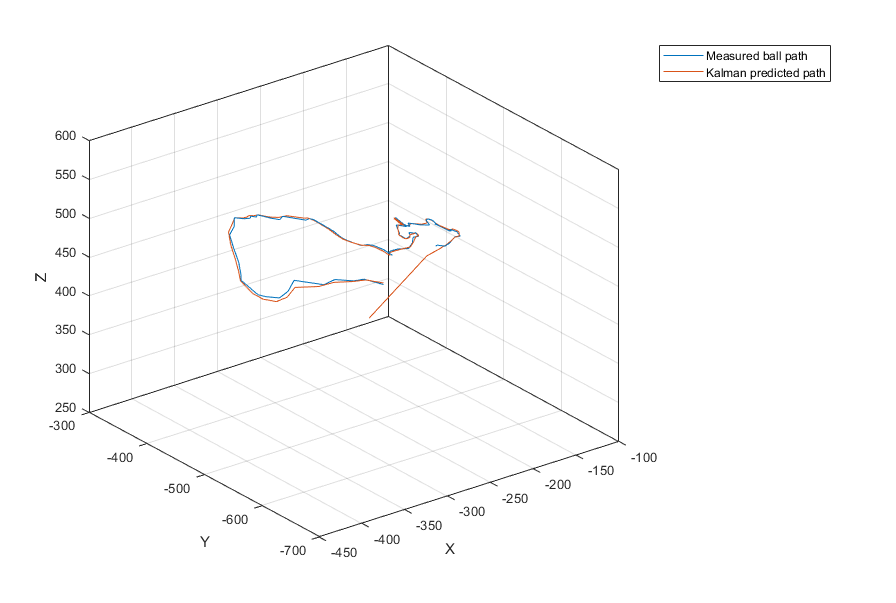
\includegraphics[width=60mm,height=60mm]{Images/kalman_plots/fourth_dyn_1.png}}
     {KF and Measurements in space.}
&
\subf{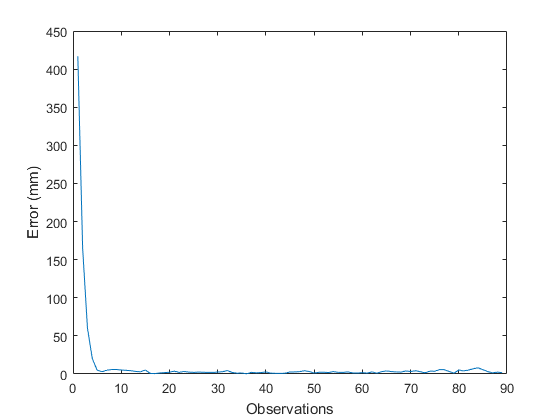
\includegraphics[width=60mm,height=60mm]{Images/kalman_plots/fourth_dyn_error.png}}
     {Kalman Filter error.}
%\hline
\end{tabular}}
\caption{Dynamic - 4: Q = 300 and R = 300.}
\label{fig:kf_dyn4}
\end{figure} 
\clearpage

\input{References.bib}

\end{document}